\section{第Vポジション}
\begin{center}
\begin{tabular}{|lcl|}
\hline
この章の基礎練習 & : & 1. 開放弦の練習 2. 「\ref{half_scale}」「\ref{1st_scale}」「\ref{2nd_scale}」「\ref{4th_scale}」「\ref{3rd_scale}」の音階練習 3. 「ます」\\
この章の修了課題 & : & 「\ref{5th_scale}」の音階練習とベートーヴェンを正しい音程で暗譜して演奏できる\\
\hline
\end{tabular}
\end{center}
\begin{flushleft}
\begin{minipage}{300pt}
\subsection{第Vポジションの位置}
\ \ \ \ 第Vポジションは第IVの半音上です。第IVポジションが隣の弦の第Iポジ
ションと同じ指に対応していたように、第Vポジションで取れる音は、細い方の隣の弦
の第IIポジションの音に対応しています。
\subsection{第Vポジションで取れる音}
\begin{music}
\nostartrule
\parindent 0pt
\setclef1{\bass}  
\startpiece
\notes\enotes
\Notes\zchar{18}{G線}\zchar{13}{\bf 1}\wh{^d}\zchar{14}{\bf 2}\wh{e}\zchar{15}{\bf 4}\wh{f}\enotes
\doublebar
\Notes\zchar{14}{\bf 1}\wh{_e}\zchar{14}{\bf 2}\wh{=e}\zchar{15}{\bf 4}\wh{f}\enotes
\doublebar
\Notes\zchar{18}{D線}\zchar{10}{\bf 1}\wh{^a}\zchar{11}{\bf 2}\wh{b}\zchar{12}{\bf 4}\wh{c}\enotes
\doublebar
\Notes\zchar{11}{\bf 1}\wh{_b}\zchar{11}{\bf 2}\wh{=b}\zchar{12}{\bf 4}\wh{c}\enotes
\setdoublebar
\endpiece
\startpiece
\notes\enotes
\Notes\zchar{14}{A線}\zchar{9}{\bf 1}\wh{'F}\zchar{9}{\bf 2}\wh{^F}\zchar{9}{\bf 4}\wh{G}\enotes
\doublebar
\Notes\zchar{9}{\bf 1}\wh{'F}\zchar{9}{\bf 2}\wh{_G}\zchar{9}{\bf 4}\wh{=G}\enotes
\doublebar
\Notes\zchar{14}{E線}\zchar{9}{\bf 1}\wh{'C}\zchar{9}{\bf 2}\wh{^C}\zchar{9}{\bf 4}\wh{D}\enotes
\doublebar
\Notes\zchar{9}{\bf 1}\wh{'C}\zchar{9}{\bf 2}\wh{_D}\zchar{9}{\bf 4}\wh{D}\enotes
\setdoublebar
\endpiece
\end{music}
\end{minipage}
\hfill
\begin{minipage}{115pt}
\addtocounter{figure}{1}
\begin{center}
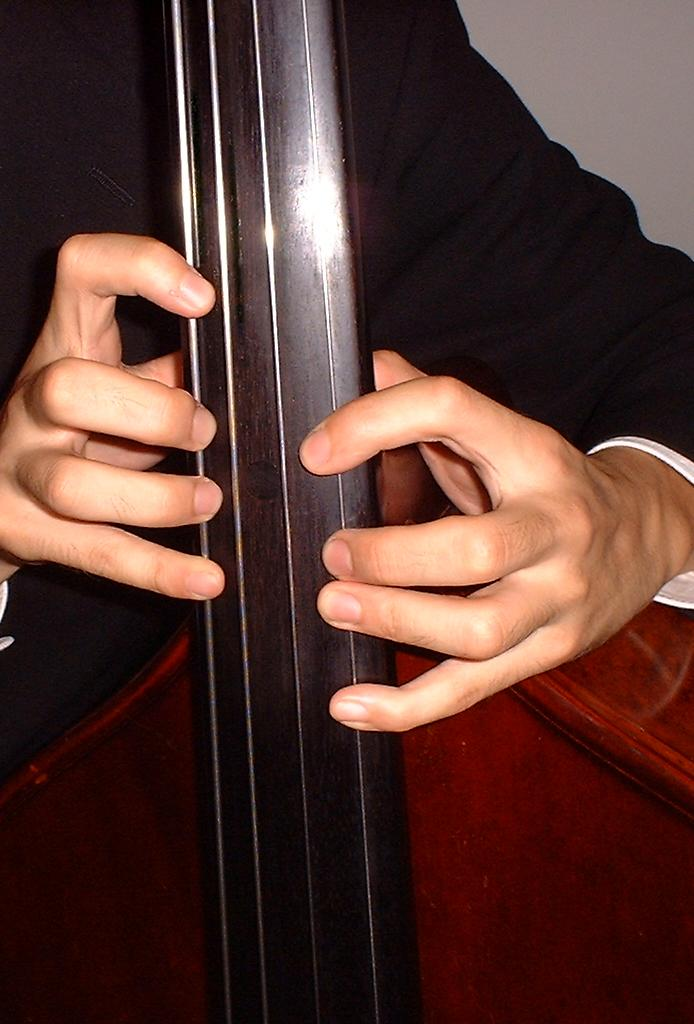
\includegraphics[width=4cm]{../Vol1/Pics/Position/5th.epsi}\\
{\flushleft\small 図\thefigure : 第Vは第IVの半音上\\}
\end{center}
\end{minipage}
\end{flushleft}

\subsection{音階練習 \label{5th_scale}}
この節からは今までの1オクターヴの音階練習に代わって、第\ref{scales}章の
音階練習を少しずつ習得していきます。長短合わせて全24の調を1つずつ
\underline{\bf 暗譜}して、一生ものの基礎練習として身に付けましょう。\\

\begin{music}
\nostartrule
\parindent 0pt
\setclef1{\bass}  
\generalsignature{-1}    
\startpiece
\notes\zchar{15}{ヘ長調(F-dur)音階}\enotes
\Notes\zchar{-6}{half}\zchar{10}{\downbow}\zchar{8}{\bf 1}\qu{F}\enotes
\notes\ibu{0}{G}{3}\islurd{0}{G}\zchar{8}{\upbow}\qb{0}{G}\tbu{0}\tslur{0}{'A}\qb{0}{A}\enotes
\notes\ibl{0}{'B}{3}\qb{0}{B}\qb{0}{C}\qb{0}{D}\tbl{0}\qb{0}{E}\enotes
\bar
\Notes\zchar{9}{\downbow}\ql{'F}\enotes
\notes\ibl{0}{'G}{3}\isluru{0}{G}\zchar{10}{\upbow}\qb{0}{G}\tbl{0}\tslur{0}{!a}\qb{0}{a}\enotes
\notes\ibl{0}{b}{3}\qb{0}{b}\zchar{-5}{III}\zchar{12}{\bf 1}\qb{0}{c}\qb{0}{d}\tbl{0}\zchar{-5}{V}\zchar{14}{\bf 2}\qb{0}{e}\enotes
\bar
\Notes\zchar{14}{\downbow}\ql{f}\enotes
\notes\ibl{0}{e}{-2}\isluru{0}{e}\zchar{14}{\upbow}\qb{0}{e}\tbl{0}\tslur{0}{d}\zchar{-5}{III}\zchar{14}{\bf 4}\qb{0}{d}\enotes
\notes\ibl{0}{c}{-3}\qb{0}{c}\zchar{-5}{half}\zchar{11}{\bf 4}\qb{0}{b}\qb{0}{a}\tbl{0}\qb{0}{'G}\enotes
\bar
\notes\ibl{0}{'F}{-3}\zchar{8}{\downbow}\qb{0}{F}\zchar{8}{\upbow}\qb{0}{E}\qb{0}{D}\tbl{0}\qb{0}{C}\enotes
\notes\ibu{0}{'B}{-3}\qb{0}{B}\qb{0}{A}\qb{0}{!G}\tbu{0}\qb{0}{F}\enotes
\endpiece

\generalsignature{-4}    
\startpiece
\notes\zchar{14}{ヘ短調(f-moll)音階}\enotes
\Notes\loffset{1}{\zchar{-5}{half}}\zchar{8}{\bf 1}\qu{F}\enotes
\notes\ibu{0}{G}{3}\islurd{0}{G}\zchar{-5}{I}\zchar{8}{\bf 2}\qb{0}{G}\tbu{0}\tslur{0}{'A}\qb{0}{A}\enotes
\notes\ibl{0}{'B}{3}\zchar{-8}{half}\zchar{8}{\bf 1}\qb{0}{B}\qb{0}{C}\qb{0}{=D}\tbl{0}\qb{0}{=E}\enotes
\bar
\Notes\ql{'F}\enotes
\notes\ibl{0}{'G}{3}\isluru{0}{G}\qb{0}{G}\tbl{0}\tslur{0}{!a}\qb{0}{a}\enotes
\notes\ibl{0}{b}{3}\qb{0}{b}\zchar{-4}{III}\zchar{12}{\bf 1}\qb{0}{c}\qb{0}{=d}\tbl{0}\zchar{-4}{V}\zchar{14}{\bf 2}\qb{0}{=e}\enotes
\bar
\Notes\ql{f}\enotes
\notes\ibl{0}{e}{-2}\isluru{0}{e}\qb{0}{_e}\tbl{0}\tslur{0}{d}\loffset{0.7}{\zchar{-5}{\small [}}\roffset{0.3}{\zchar{-4}{\small II}}\zchar{-7}{\small III}\zchar{14}{\bf 4}\qb{0}{_d}\enotes
\notes\ibl{0}{c}{-3}\qb{0}{c}\zchar{-4}{half}\zchar{12}{\bf 4}\qb{0}{b}\qb{0}{a}\tbl{0}\qb{0}{'G}\enotes
\bar
\notes\ibl{0}{'F}{-3}\qb{0}{F}\qb{0}{E}\zchar{-6}{I}\zchar{8}{\bf 4}\qb{0}{D}\tbl{0}\qb{0}{C}\enotes
\notes\ibu{0}{'B}{-3}\loffset{1.4}{\zchar{-4}{half}}\zchar{10}{\bf 1}\qb{0}{B}\roffset{0.3}{\zchar{-4}{I}}\zchar{10}{\bf 4}\qb{0}{A}\qb{0}{!G}\tbu{0}\zchar{-5}{half}\zchar{8}{\bf 1}\qb{0}{F}\enotes
\endpiece

\generalsignature{-5}    
\startpiece
\notes\zchar{14}{変ロ短調(b-moll)音階}\enotes
\Notes\loffset{1}{\zchar{-4}{half}}\zchar{8}{\bf 1}\qu{'B}\enotes
\notes\ibu{0}{'C}{3}\islurd{0}{C}\zchar{-4}{I}\zchar{8}{\bf 2}\qb{0}{C}\tbu{0}\tslur{0}{D}\qb{0}{D}\enotes
\notes\ibl{0}{'E}{3}\zchar{-5}{half}\zchar{8}{\bf 1}\qb{0}{E}\qb{0}{F}\qb{0}{=G}\tbl{0}\qb{0}{=!a}\enotes
\bar
\notes\ibl{0}{b}{0}\isluru{0}{b}\qb{0}{b}\tslur{0}{a}\qb{0}{=a}\qb{0}{b}\tbl{0}\loffset{0.7}{\zchar{-5}{\small [}}\roffset{0.3}{\zchar{-4}{\small II}}\zchar{-7}{\small III}\zchar{12}{\bf 2}\qb{0}{c}\enotes
\notes\ibl{0}{d}{0}\isluru{0}{d}\qb{0}{d}\tslur{0}{c}\qb{0}{c}\qb{0}{d}\tbl{0}\zchar{-4}{V}\zchar{14}{\bf 1}\qb{0}{e}\enotes
\bar
\notes\ibl{0}{f}{-3}\isluru{0}{f}\qb{0}{f}\tslur{0}{e}\qb{0}{e}\loffset{0.7}{\zchar{-5}{\small [}}\roffset{0.3}{\zchar{-4}{\small II}}\zchar{-7}{\small III}\zchar{13}{\bf 4}\qb{0}{d}\tbl{0}\qb{0}{c}\enotes
\notes\ibl{0}{d}{-3}\isluru{0}{d}\qb{0}{d}\tslur{0}{c}\qb{0}{c}\zchar{-4}{half}\zchar{11}{\bf 4}\qb{0}{b}\tbl{0}\qb{0}{=a}\enotes
\bar
\notes\ibl{0}{b}{-3}\qb{0}{b}\qb{0}{_a}\zchar{-4}{I}\zchar{9}{\bf 4}\qb{0}{'_G}\tbl{0}\qb{0}{F}\enotes
\notes\ibu{0}{'E}{-3}\loffset{1}{\zchar{-4}{half}}\zchar{1}{\bf 1}\qb{0}{E}\roffset{0.4}{\zchar{-4}{I}}\zchar{0}{\bf 4}\qb{0}{D}\qb{0}{C}\tbu{0}\zchar{-5}{half}\zchar{-2}{\bf 1}\qb{0}{B}\enotes
\endpiece
\end{music}

\subsection{第Vポジションまでで弾ける名曲}
\documentclass{jarticle}
\usepackage{musixdoc}
\startmuflex\makeindex

\begin{document}

\subsubsection*{����������ǥ�: ������������նʡֽ�����1�ھϤ��}
\begin{music}
\nostartrule
\setclef1{\bass}
\generalsignature{-1}    
\generalmeter{\meterC}
\parindent 0pt
\startbarno=17
\def\writebarno{\tenrm\the\barno\barnoadd}
\def\raisebarno{2\internote}
\def\shiftbarno{0.1\Interligne}
\systemnumbers
\startpiece\bigaccid
\notes\zchar{16}{\bf (Allegro)}\enotes
\notes\ibl{0}{d}{0}\qb{0}{f}\qb{0}{f}\qb{0}{f}\tbl{0}\qb{0}{c}\enotes
\Notes\ql{f}\enotes
\notes\ibl{0}{d}{-2}\qb{0}{f}\tbl{0}\qb{0}{c}\enotes
\bar
\notes\ibl{0}{d}{0}\qb{0}{f}\qb{0}{f}\qb{0}{f}\tbl{0}\qb{0}{c}\enotes
\Notes\ql{f}\enotes
\notes\ibl{0}{d}{-2}\qb{0}{f}\tbl{0}\qb{0}{c}\enotes
\bar
\notes\ibl{0}{d}{-1}\qb{0}{f}\qb{0}{f}\qb{0}{b}\tbl{0}\qb{0}{=b}\enotes
\Notes\ql{c}\qp\enotes
\bar
\notes\ibl{0}{d}{0}\qb{0}{f}\qb{0}{f}\qb{0}{f}\tbl{0}\qb{0}{f}\enotes
\Notes\ql{b}\enotes
\notes\ibl{0}{'E}{4}\qb{0}{F}\tbl{0}\qb{0}{!f}\enotes
\bar
\notes\ibl{0}{d}{0}\qb{0}{f}\qb{0}{f}\qb{0}{f}\tbl{0}\qb{0}{f}\enotes
\Notes\ql{b}\enotes
\notes\ibl{0}{'E}{4}\qb{0}{F}\tbl{0}\qb{0}{!f}\enotes
\bar
\Notes\ql{b}\enotes
\notes\ibl{0}{'F}{4}\qb{0}{F}\tbl{0}\qb{0}{!f}\enotes
\Notes\ql{f}\ql{e}\enotes
\bar
\Notes\ql{f}\ql{c}\ql{'F}\qp\enotes
\setdoublebar
\endpiece
\end{music}

\endmuflex
\end{document}

\documentclass{jarticle}
\usepackage{musixdoc}
\startmuflex\makeindex

\begin{document}

\subsubsection*{���塼�ޥ�: �������1�� ��1�ھ���Ƭ}

\begin{music}
\nostartrule
\setclef1{\bass}  
\generalsignature{-1}    
\generalmeter{\meterfrac34}
\parindent 0pt
\startbarno=1
\def\writebarno{\tenrm\the\barno\barnoadd}
\def\raisebarno{2\internote}
\def\shiftbarno{0.1\Interligne}
\systemnumbers
\startpiece\bigaccid
\notes\zchar{17}{\bf Molto vivace}\enotes
\Notes\ql{'D}\enotes
\bar
\barno=1
\Notes\hlp{'G}\enotes
\bar
\Notes\ql{'D}\qp\ql{=F}\enotes
\bar
\Notes\hlp{b}\enotes
\bar
\Notes\ql{'F}\qp\ql{!a}\enotes
\bar
\Notes\hl{'D}\ql{E}\enotes
\bar
\Notes\ql{'E}\ql{E}\ql{F}\enotes
\bar
\Notes\hl{'G}\ql{G}\enotes
\bar
\Notes\ql{a}\qp\ql{a}\enotes
\bar
\Notes\hlp{d}\enotes
\bar
\Notes\ql{a}\qp\ql{=c}\enotes
\bar
\Notes\hlp{f}\enotes
\bar
\Notes\ql{c}\qp\ql{d}\enotes
\bar
\Notes\hl{'G}\ql{!a}\enotes
\bar
\Notes\ql{a}\ql{a}\ql{b}\enotes
\bar
\Notes\hl{a}\ql{a}\enotes
\bar
\Notes\ql{'D}\qp\enotes
\setrightrepeat
\endpiece
\end{music}

\endmuflex
\end{document}

\documentclass{jarticle}
\usepackage{musixdoc}
\startmuflex\makeindex

\begin{document}

\subsubsection*{���㥤���ե�����: �֥�����Կʶʡפ��}
\begin{music}
\nostartrule
\setclef1{\bass}  
\generalsignature{-5}    
\generalmeter{\meterC}
\parindent 0pt
\startbarno=66
\def\writebarno{\tenrm\the\barno\barnoadd}
\def\raisebarno{2\internote}
\def\shiftbarno{0.1\Interligne}
\systemnumbers
\startpiece\bigaccid
\notes\zchar{17}{\bf (Moderato in modo di marcia funebre)}\enotes
\Notes\hl{f}\ql{=e}\ibl{0}{d}{-2}\qb{0}{d}\tbl{0}\qb{0}{c}\enotes
\bar
\Notes\hlp{b}\ibl{0}{c}{2}\qb{0}{c}\tbl{0}\qb{0}{d}\enotes
\bar
\Notes\ql{ff=e}\ibl{0}{d}{-2}\qb{0}{d}\tbl{0}\qb{0}{c}\enotes
\bar
\Notes\wh{b}\enotes
\bar
\Notes\ql{c_edc}\enotes
\bar
\Notes\ibl{0}{d}{-2}\qb{0}{d}\tbl{0}\qb{0}{c}\enotes
\bar
\notes\multnoteskip\tinyvalue\tinynotesize\ibu{0}{b}{2}\ibbu{0}{b}{2}\qb{0}{b}\tbbu{0}\tbu{0}\qb{0}{c}\enotes
\Notes\ibl{0}{b}{-2}\qb{0}{b}\tbl{0}\qb{0}{=a}\ibl{0}{b}{2}\qb{0}{b}\tbl{0}\qb{0}{c}\ql{db}\enotes
\bar
\Notes\ibl{0}{f}{0}\qb{0}{f}\tbl{0}\qb{0}{f}\ql{=ed}\ibl{0}{c}{-2}\qb{0}{c}\tbl{0}\qb{0}{b}\enotes
\bar
\Notes\ibl{0}{f}{0}\qb{0}{f}\tbl{0}\qb{0}{f}\ql{=ed}\ibl{0}{c}{-2}\qb{0}{c}\tbl{0}\qb{0}{b}\enotes
\bar
\Notes\ibl{0}{f}{-3}\qb{0}{f=ed}\tbl{0}\qb{0}{b}\enotes
\Notes\ibl{0}{f}{-3}\qb{0}{f=ed}\tbl{0}\qb{0}{b}\enotes
\bar
\Notes\ibl{0}{'F}{-4}\qb{0}{!f}\tbl{0}\qb{0}{'B}\ibu{0}{B}{0}\qb{0}{B}\tbu{0}\qb{0}{B}\ibu{0}{B}{0}\qb{0}{BBB}\tbu{0}\qb{0}{B}\enotes
\bar
\Notes\cu{'B}\ds\qp\hp\enotes
\mulooseness=0
\setdoublebar
\endpiece
\end{music}

\endmuflex
\end{document}


\clearpage

\subsection{豆知識: コントラバス3大名人}
ヴァイオリンのパガニーニやサラサーテほどには広く知られていませんが、コン
トラバス演奏の歴史にも伝説的名人が3人ほど存在します。3人ともコントラバ
ス協奏曲を作曲するなど、コントラバス独奏曲のレパートリーを語る上で欠か
せない存在です。

\subsubsection*{ドメニコ・ドラゴネッティ(Domenico Dragonetti, 1763-1846)}
イタリアのヴェネツィア生まれ。ベートーヴェンが自ら指揮した交響曲第7番
の初演に参加したり、ロッシーニから「チェロとコントラバスのための二重奏
曲」を贈られるなど、同時代を生きていた大作曲家たちと親交がありました。
ベートーヴェンはそれまでチェロの補助楽器程度にしか扱われていなかったコ
ントラバスの役割を大幅に拡大していますが、これはドラゴネッティの演奏技
巧を実際に目の当たりにしたことの影響であると考えられています。前ページ
の交響曲第5番からの抜粋はその好例と言えるでしょう。\\
\indent ドラゴネッティは現在「ジャーマン・ボウ」と呼ばれている弓の成立
に関わり、広めた人でもあります。現在、ジャーマン・ボウはライン川から東の
ヨーロッパや日本で多く使われています。本書で紹介したのもジャーマン・ボ
ウです。\\
\indent 性格は相当変わっていたらしく、等身大のマネキンに服を着せて演奏
旅行先まで一緒に持って行き、コンサートホールの最前列に座らせ、あげくの
果てには楽屋を訪ねて来た友人たちに「これが妻で、それが息子で・・・」と
紹介したとか。

\subsubsection*{ジョヴァンニ・ボッテシーニ(Giovanni Bottesini, 1821-89)}
イタリアのクレマ(ミラノ近郊)生まれ。ミラノ音楽院に入学する際、「奨学金
の枠が残っているのはファゴットとコントラバスだけ」と言われてコントラバ
スを選択したと伝えられています。指揮者としても有能だったようで、ヴェル
ディからオペラ「アイーダ」の初演を任されています。\\
\indent 「ジャーマン・ボウ」はドラゴネッティによって広まりましたが、ボッ
テシーニはチェロの弓と同じ持ち方をするいわゆる「フレンチ・ボウ」を用い
て独奏を行い、ベルリオーズ(「幻想交響曲」の作曲家)に評価されました。フ
レンチ・ボウはライン川から西のヨーロッパや英語圏で多く使われています。
\\
\indent ボッテシーニが愛用した弓には''Il Devastatore (破壊者)''という
名が付いています。逸話によれば、コントラバスが通らないほど狭いドアの枠
をボッテシーニがこの弓で叩き壊したのが「破壊者」という名の由来とのこと
です。真似しないように。

\subsubsection*{セルゲイ・クーセヴィツキー(Serge Koussevitzky, 1874-1951)}

ロシアのヴィシュニ・ヴォロチョク(モスクワとサンクトペテルブルグの間)生
まれ。モスクワ音楽院を卒業し、最初はコントラバス奏者として、後に指揮者
としても活躍しました。ロシア革命後はアメリカに亡命し、ボストン交響楽団
を世界的なオーケストラに育てています。指揮者としてはミスをした楽員をそ
の場でクビにするなどかなりの暴君だったようですが、ボストン交響楽団との
関係は25年の長きにわたって続きました。\\
\indent 上記2人の名人と同様に同時代の大作曲家と交流を持ち、バルトーク
に「管弦楽のための協奏曲」を、ラヴェルにはピアノ組曲「展覧会の絵」(ム
ソルグスキー作曲)のオーケストレーションを委嘱し、ボストン交響楽団を指
揮してそれぞれ初演しています。\\
\indent また、マサチューセッツ州のタングルウッドに現在まで続く音楽祭を
創設し、ここでは若き日のレナード・バーンスタイン(指揮者・作曲家)を指導
しています。バーンスタインの交響曲第2番「不安の時代」はクーセヴィツキー
が初演を指揮しました。\\
\indent 同音楽祭では「クーセヴィツキー大賞」を優秀な若手指揮者に贈って
います。有名なところではクラウディオ・アバドや小澤征爾が受賞しており、
後にそれぞれベルリン・フィルやウィーン国立歌劇場の監督になっています。
現代の指揮者の系譜に大きな影響を与えた音楽家だったとも言えましょう。
\\
